%\documentclass[10pt,a4paper]{article}
\documentclass[10pt,a4paper]{scrreprt}
\usepackage[utf8]{inputenc}
\usepackage{amsmath}
\usepackage{amsfonts}
\usepackage{amssymb}
\usepackage{graphicx}
\usepackage[left=2cm,right=2cm,top=2cm,bottom=2cm]{geometry}

\usepackage{bm}
\usepackage{natbib}

% integral d
\newcommand{\myd}{\;\mathrm{d}}
% overbar
\newcommand{\overbar}[1]{\mkern 1.5mu\overline{\mkern-1.5mu#1\mkern-1.5mu}\mkern 1.5mu}

\author{Yi Hu}
\title{Homogenization for Multi Field Modelling}
\subtitle{Part I: Theories and FEniCS}


\begin{document}

\chapter{Homogenization Method}
The method used in the current work is Homogenization Method. It was proposed in 1970s by Babuska and collaborators \citep{EPFL-ARTICLE-184958}. The main purpose of this method is to make use of the scale separation, in order that a reduced PDE for the macroscopic problem is obtained. The macroscopic problem always contains the information from the corresponding micro scale, and it is often represented as ``effective parameters''. These effective parameters are often calculated in the sense of ``averaging procedure'' or ``homogenization''. In order to obtain homogenized quantities a micro scale problem needs to be solved. It could be solved with numerical methods such as Finite Element Method, Finite Volume Method or theoretical results in simple cases. An extensive review  can be found in book \citep{efendiev2009multiscale}. A more general framework, the Heterogeneous Multiscale Method (HMM), was proposed by Bjorn Engquist. This method extend the idea of homogenization and introduce generic methodology between macro scale and micro scale. An introductory review could be found in \citep{weinan2007heterogeneous}.

In this part the basic idea of Homogenization Method is presented with a one dimensional example. Then the application to the 3D elliptic PDE is briefly discussed. Hill Mandel requirements should be fulfilled in the energy conserving problem. Hence they are stated in the end of this part. We confine our discussion here mainly on materials with periodic structures. 

\section{Periodic Structures}
Periodicity appears frequently in composites, for instance material with fiber or particle reinforcement. In these materials inclusions are arranged periodically. Concerning about material parameters they could be expressed with periodic functions of coordinates. For example, Young's Modulus can be written in the following form,
%
\begin{equation}
\label{eq:periodic 1}
\mathbb{C}(\mathbf{x}+\mathbf{Y}) = \mathbb{C}(\mathbf{x}).
\end{equation}
%

\section{Scale Separation}
When a two scale problem is addressed, a corresponding field variable could be expanded as follows, 
%
\begin{equation}
\label{eq:field epsi}
\mathbf{\Phi}^{\epsilon}(\mathbf{x}) = \mathbf{\Phi}^{0}(\mathbf{x},\mathbf{y}) + \epsilon\mathbf{\Phi}^{1}(\mathbf{x},\mathbf{y}) + \epsilon\mathbf{\Phi}^{2}(\mathbf{x},\mathbf{y}) + \cdots,
\end{equation}
%
In the above formula, $\mathbf{x}$ is the position vector of a point, which is deemed as the \textit{macroscopic} coordinate. $\mathbf{y}=\mathbf{x}/\epsilon$ is a \textit{microscopic} coordinate, which stands for \textit{rapid} oscillation. The physical nature of the right hand side is the decomposition of macro scale dependency and micro scale dependency with respect to a reference cell. The purpose of setting $\mathbf{y}=\mathbf{x}/\epsilon$ is achieving a closed form expressed with the original coordinates. The ratio $\epsilon$ means that the micro quantity will vary $1/\epsilon$ faster than macroscopic level. When $\epsilon$ goes to $0$, functions $\mathbf{\Phi}^{0}(\mathbf{x}, \mathbf{y}), \mathbf{\Phi}^{1}(\mathbf{x}, \mathbf{y}), \cdots$ are smooth in $\mathbf{x}$ and $\mathbf{Y}$-periodic in $\mathbf{y}$.

The characteristic of field variable is illustrated in the following figure.

\begin{figure}[h]
  \centering
    \label{fig: scale sepa}
    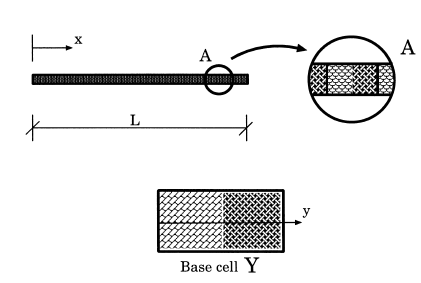
\includegraphics[width=0.45\linewidth]{../pics/ref_cell_mic_mac_coord.png}
  \caption{Micro and Macro Coordinate of Field Variable \citep{hassani1998review}}
\end{figure}

\section{One Dimensional Problem}
Many books and review papers list one dimensional problem, such as \citep{cioranescu2000introduction}. Here we briefly go through one dimensional elasticity problem. More detailed derivation could be referred to \citep{hassani1998review}.

The governing equations, i.e. the equilibrium and Hooke's law are,
\begin{equation}
\left\{
\begin{array}{l}
\dfrac{\partial \sigma^{\epsilon}}{\partial x} + \gamma^{\epsilon} = 0 \\
\sigma^{\epsilon} = E^{\epsilon} \dfrac{\partial u^{\epsilon}}{\partial x},
\end{array}
\right.
\end{equation}

Noting that $\epsilon$ in superscript represents its periodic property. $\gamma^{\epsilon}$ is the body weight of material. If $E^{\epsilon}$ and $\gamma^{\epsilon}$ are uniform in macro coordinate and only differ inside each cell, then the following relation holds,
\begin{equation}
E^{\epsilon}(x,x/\epsilon)=E^{\epsilon}(x/\epsilon)=E(y),
\end{equation}
The relation with respect to body weight is likewise. Regarding the double scale expansion according to (\ref{eq:field epsi}) it follows,
\begin{equation}
\left\{
\begin{array}{l}
u^{\epsilon}(x) = u^{0}(x,y) + \epsilon u^{1}(x,y) + \epsilon^{2} u^{2}(x,y) + \cdots \\
\sigma^{\epsilon}(x) = \sigma^{0}(x,y) + \epsilon \sigma^{1}(x,y) + \epsilon^{2} \sigma^{2}(x,y) + \cdots,
\end{array}
\right.
\end{equation}

After substitution and equating the correspondent terms, we have
\begin{equation}
\label{eq: to simp 1}
\left\{
\begin{array}{l}
0 = E(y)\left( \dfrac{\partial u^{0}}{\partial y} \right) \\
\sigma^{0} = E(y) \left( \dfrac{\partial u^{0}}{\partial x} + \dfrac{\partial u^{1}}{\partial y} \right) \\
\sigma^{1} = E(y) \left( \dfrac{\partial u^{1}}{\partial x} + \dfrac{\partial u^{2}}{\partial y} \right),
\end{array}
\right.
\end{equation}
and
\begin{equation}
\label{eq: to simp 2}
\left\{
\begin{array}{l}
\dfrac{\partial \sigma^{0}}{\partial y}=0 \\
\dfrac{\partial \sigma^{0}}{\partial x} + \dfrac{\partial \sigma^{1}}{\partial y} + \gamma(y) = 0, 
\end{array}
\right.
\end{equation}
Simplification of (\ref{eq: to simp 1}) and (\ref{eq: to simp 2}) yields
\begin{equation}
\label{eq: sigma 0}
\sigma^{0}(x) = \left(Y/\int_{Y} \dfrac{\myd{y}}{E(y)} \right) \dfrac{\myd{u^{0}(x)}}{\myd{x}}.
\end{equation}
Define the \textit{homogenized modulus of elasticity} as follows,
\begin{equation}
E^{H} = 1/ \left( \dfrac{1}{Y} \int_{0}^{Y} \dfrac{\myd{\eta}}{E(\eta)}\right) .
\end{equation}
Then the original problem is transformed to
\begin{equation}
\label{eq: homo 1d}
\left\{
\begin{array}{l}
\sigma^{0}(x) = E^{H} \dfrac{\myd{u^{0}(x)}}{\myd{x}} \\
\dfrac{\myd{\sigma^{0}}}{\myd{x}} + \bar{\gamma} = 0,
\end{array}
\right.
\end{equation}
where $\bar{\gamma}=1/Y \int_{Y} \gamma(y)$ is the average of $\gamma$ inside the cell. From (\ref{eq: homo 1d}) the differential equation for displacement holds as
\begin{equation}
\dfrac{\myd^2 u^{0}(x)}{\myd{x^{2}}} = -\dfrac{\bar{\gamma}}{E^{H}}
\end{equation}
Accounting the boundary conditions on both ends gives the result
\[u(x) = -\dfrac{\bar{\gamma}}{E^{H}} \dfrac{x^{2}}{2} + \dfrac{\bar{\gamma}}{E^{H}} Lx \]

\section{General Elliptical PDE}
If a general PDE for three dimensional problem is taken into account, it would be more intricate, as the solution is often sought in the sense of weak form. In this circumstance a homogenized weak form is considered instead of the homogenized differential operator. Then the limit of homogenized weak form should converge to the weak form without homogenization, which is called \textit{G-convergence}, \citep{hollister1992comparison}. As for the case of elasticity tensor in the sense of differential operator G-convergence is expressed as
\begin{equation}
\label{eq: G conv}
\lim_{\epsilon \to 0} \dfrac{\partial}{\partial x_{i}} \left[ C^{\epsilon}_{ijkl} \dfrac{\partial u^{\epsilon}_{k}}{\partial x_{l}} \right] \rightarrow \dfrac{\partial}{\partial x_{i}} \left[ \bar{C}_{ijkl} \dfrac{\partial u_{k}}{\partial x_{l}} \right]
\end{equation}
A quick overview of the general problem is given in the review \citep{hassani1998review}. Several key points of the general problem are listed here. With the notation of general elliptical operator using 
\begin{equation}
\mathcal{A}^{\epsilon} = \dfrac{\partial}{\partial x_{i}} \left( a_{ij}(\mathbf{y}) \dfrac{\partial}{\partial x_{j}} \right).
\end{equation}
general problem could then be described as,
\begin{equation}
\left\{
\begin{array}{ll}
\mathcal{A}^{\epsilon} \mathbf{u^{\epsilon}}= \mathbf{f} & \text{in} \ \Omega \\
\mathbf{u}^{\epsilon} = \mathbf{0} & \text{on} \ \partial \Omega
\end{array}
\right.
\end{equation}
Employing the double scale expansion for both the field variable $\mathbf{u}^{\epsilon}$ and the differential operator $\mathcal{A}^{\epsilon}$, namely (notice that chain rule is applied when differentiating)
\begin{equation}
\left\{
\begin{array}{l}
\mathbf{u}^{\epsilon}(\mathbf{x}) = \mathbf{u}^{0}(\mathbf{x},\mathbf{y}) + \epsilon \mathbf{u}^{1}(\mathbf{x},\mathbf{y}) + \epsilon^{2} \mathbf{u}^{2}(\mathbf{x},\mathbf{y}) + \cdots \\
\mathcal{A}^{\epsilon} = \dfrac{1}{\epsilon^{2}} \mathcal{A}^{1} + \dfrac{1}{\epsilon} \mathcal{A}^{2} + \mathcal{A}^{3}
\end{array}
\right.
\end{equation}
Here $\mathcal{A}^{1}, \mathcal{A}^{2}, \mathcal{A}^{3}$ is defined as follows
\[
\mathcal{A}^{1} = \dfrac{\partial}{\partial y_{i}} \left( a_{ij}(\mathbf{y}) \dfrac{\partial}{\partial y_{j}} \right); \
\mathcal{A}^{2} = \dfrac{\partial}{\partial y_{i}} \left( a_{ij}(\mathbf{y}) \dfrac{\partial}{\partial x_{j}} \right) + \dfrac{\partial}{\partial y_{i}} \left( a_{ij}(\mathbf{y}) \dfrac{\partial}{\partial x_{j}} \right); \
\mathcal{A}^{3} = \dfrac{\partial}{\partial x_{i}} \left( a_{ij}(\mathbf{y}) \dfrac{\partial}{\partial x_{j}} \right).
\]
Substitution with the above differential operators and comparing with the according terms it follows
\begin{equation}
\label{eq: eq group}
\left\{
\begin{array}{l}
\mathcal{A}^{1} \mathbf{u}^{0} = \mathbf{0} \\
\mathcal{A}^{1} \mathbf{u}^{1} + \mathcal{A}^{2} \mathbf{u}^{0} = \mathbf{0} \\
\mathcal{A}^{1} \mathbf{u}^{2} + \mathcal{A}^{2} \mathbf{u}^{1} + \mathcal{A}^{3} \mathbf{u}^{0} = \mathbf{f}.
\end{array}
\right.
\end{equation}
Referring \citep{cioranescu2000introduction} it is known that if a $\mathbf{Y}$-periodic function $u$ has a unique solution in terms of $\mathcal{A}^{1}$ operator, i.e. 
\begin{equation}
\mathcal{A}^{1} \mathbf{u} = \mathbf{F} \quad \text{in reference cell}.
\end{equation}
Then the right hand side of the above equation, $\mathbf{F}$ should satisfy 
\begin{equation}
\overbar{\mathbf{F}} = \dfrac{1}{|Y|}\int_{Y} \mathbf{F} \myd{\mathbf{y}} = \mathbf{0}.
\end{equation}
Applying this proposition to (\ref{eq: eq group}) several times the field variable could be expressed with the following form,
\begin{equation}
\mathbf{u}^{1}(\mathbf{x}, \mathbf{y}) = \chi^{i}(\mathbf{y}) \dfrac{\partial \mathbf{u}(\mathbf{x})}{\partial x_{j}} + \mathbf{\xi} (\mathbf{x})
\end{equation}
Function $\chi^{i}(\mathbf{y})$ is the local solution of this problem, which has $\mathbf{Y}$-periodic property. The local problem is
\begin{equation}
\mathcal{A}^{1} \mathbf{\chi}^{j}(\mathbf{y}) = \dfrac{\partial a_{ij}(\mathbf{y})}{\partial y_{i}} \quad \text{in reference cell}.
\end{equation}
Hence the macro scale problem (homogenized problem) can be written as
\begin{equation}
\mathcal{A}^{H} \mathbf{u} = \mathbf{f},
\end{equation}
with
\begin{equation}
\mathcal{A}^{H} = a^{H}_{ij} \dfrac{\partial^{2}}{\partial x_{i} \partial x_{j}}.
\end{equation}
%
And the effective coefficients are related with the solution of micro scale problem, i.e.
\begin{equation}
a^{H}_{ij} = \dfrac{1}{|Y|} \int_{Y} \left( a_{ij}(\mathbf{y}) + a_{ik}(\mathbf{y}) \dfrac{\partial \chi^{j}}{\partial y_{k}} \right) \myd{\mathbf{y}}
\end{equation}

%--------------------------------
\section{Hill-Mandel Condition}
After introducing the general mathematical concepts about homogenization methods, we move to its application in material modelling. In this case a Representative Volume Element (RVE) is always investigated. Homogenization of the coefficients is then obtained through calculation on RVE. As RVE represents a material in the micro scale, the behaviour of RVE should resemble the material in this scale. Therefore the model for micro scale should be able to capture specific features, for instance the continuum mechanical equilibrium of composites in the micro scale. Besides the boundary condition of micro scale model should also be compatible with macro scale. This is the content of  Hill-Mandel condition \citep{gluge2012comparison}.

The Hill-Mandel condition states that the total stress power on the micro scale should be equal to the stress power at relevant point on the macro scale. For small strain, the following equation holds,

\begin{equation}
\left< \bm{\sigma} \cdot \dot{\bm{\varepsilon}} \right> = \left< \bm{\sigma} \right> \cdot \left< \dot{\bm{\varepsilon}} \right>,
\end{equation}
where $\left< \cdot \right>$ means averaging of the considered variable. In simulations certain boundary conditions are devised to fulfil Hill-Mandel condition automatically. 

%\bibliographystyle{plain}
%\bibliography{/home/yihu/studien_arbeit_fenics/report/part1/part1_ref.bib}
%\nocite{*}

\end{document}



















